\documentclass{article}
%Packages
\usepackage{tikz}
\usetikzlibrary{shapes,arrows, positioning}


\begin{document}

\section{How to Draw the Shapes in Latex}

% DRAW RECTANGLE NODE
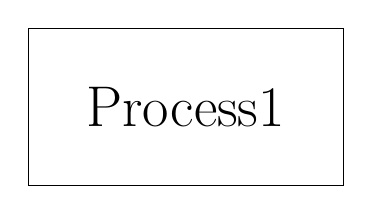
\begin{tikzpicture}
	\tikzstyle{every node}=[font=\huge]

	\node[draw,
	minimum width=4cm,
	minimum height=2cm] {Process1}; % Bydefault if you simply write as a Draw, so this means a rectangle,
% and if you wamt to fixed the width of the rectangle... you have to set minimum width, and if you want to fixed the height of the rectangle write minimum height.
% ;(semi colon) is very important.	
\end{tikzpicture}

%CHANGE LINE COLOR

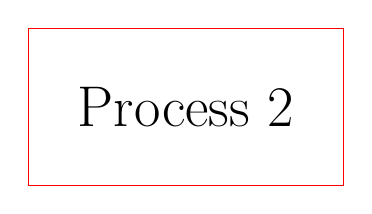
\begin{tikzpicture}


	\tikzstyle{every node}=[font=\huge]
	\node[draw=red,
	minimum width=4cm,
	minimum height=2cm]{Process 2}; % here boundary color is red instead of black, So you have to put the command draw=red,
\end{tikzpicture}

%CHANGE FILLING COLOR
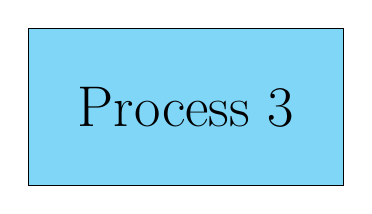
\begin{tikzpicture}

	\tikzstyle{every node}=[font=\huge]			
	\node[draw,
	fill=cyan!50,
	minimum width=4cm,
	minimum height=2cm]{Process 3}; % if yoy want to fill the color , here i use color cyan and 50% i use.
 \end{tikzpicture}

%CHANGE TEXT COLOR
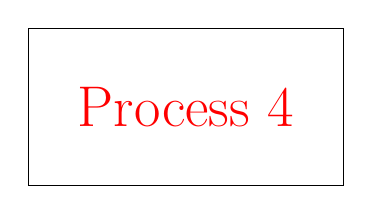
\begin{tikzpicture}
\tikzstyle{every node}=[font=\huge]
	\node [draw,
	text=red,
	minimum width=4cm,
	minimum height=2cm]{Process 4}; % if you want to add text color then , here i want red color so text=red will be the command.
\end{tikzpicture}


\end{document}


